%; whizzy paragraph -pdf xpdf -latex ./whizzypdfptex.sh
%; whizzy-paragraph "^\\\\begin{frame}"
% latex beamer presentation.
% platex, latex-beamer $B$G%3%s%Q%$%k$9$k$3$H$rA[Dj!#(B 

%     Tokyo Debian Meeting resources
%     Copyright (C) 2009 Junichi Uekawa
%     Copyright (C) 2010 Nobuhiro Iwamatsu

%     This program is free software; you can redistribute it and/or modify
%     it under the terms of the GNU General Public License as published by
%     the Free Software Foundation; either version 2 of the License, or
%     (at your option) any later version.

%     This program is distributed in the hope that it will be useful,
%     but WITHOUT ANY WARRANTY; without even the implied warranty of
%     MERCHANTABILITY or FITNESS FOR A PARTICULAR PURPOSE.  See the
%     GNU General Public License for more details.

%     You should have received a copy of the GNU General Public License
%     along with this program; if not, write to the Free Software
%     Foundation, Inc., 51 Franklin St, Fifth Floor, Boston, MA  02110-1301 USA

\documentclass[cjk,dvipdfm,12pt]{beamer}
\usetheme{Tokyo}
\usepackage{monthlypresentation}
%  preview (shell-command (concat "evince " (replace-regexp-in-string "tex$" "pdf"(buffer-file-name)) "&"))
%  presentation (shell-command (concat "xpdf -fullscreen " (replace-regexp-in-string "tex$" "pdf"(buffer-file-name)) "&"))
%  presentation (shell-command (concat "evince " (replace-regexp-in-string "tex$" "pdf"(buffer-file-name)) "&"))

%http://www.naney.org/diki/dk/hyperref.html
%$BF|K\8l(BEUC$B7O4D6-$N;~(B
\AtBeginDvi{\special{pdf:tounicode EUC-UCS2}}
%$B%7%U%H(BJIS$B7O4D6-$N;~(B
%\AtBeginDvi{\special{pdf:tounicode 90ms-RKSJ-UCS2}}

\title{upstart $B:FF~Lg(B}
\subtitle{}
\author{$BA0ED(B $B9LJ?(B mkouhei@debian.or.jp\\IRC nick: mkouhei}
\date{2010$BG/(B4$B7n(B17$BF|(B}
\logo{
\includegraphics[width=8cm]{image200607/openlogo-light.eps}}

\begin{document}

\frame{\titlepage{}}

\begin{frame}
 \frametitle{$B?<F~$j$7$h$&$H$7$?$N$@$,!D!#(B}

  \begin{itemize}
   \item $B;EAH$_$N?<F~$j$r;n$_$?$N$@$,!D!#(B
   \item $BG/EYJQ$o$C$F%W%i%$%Y!<%H$NM>NO$,$J$/$F:C@^!#(B
   \item 2$B7n$H$^$C$?$/F1$8$N$b$I$&$+$H!#(B
  \end{itemize}
 $B$=$3$G(Bupstart$B$N5/F0$r(B bootchart $B$G8+$F$_$?!#(B
\end{frame}


\section{}
\begin{frame}
 \frametitle{$B;vA0=`Hw(B}
 $BMQ0U$9$k(B $B%$%s%9%H!<%k%$%a!<%8!"%Q%C%1!<%8!"(B
 \begin{itemize}
  \item debian-testing-amd64-businesscard.iso
  \item qemu-kvm $B%Q%C%1!<%8(B
  \item qcow2 $B%U%)!<%^%C%H$N%G%#%9%/%$%a!<%8(B
  \item bootchart $B%Q%C%1!<%8(B
 \end{itemize}

 KVM/QEMU $B%2%9%H$K(B sysvinit $B$H(B upstart $B$N(B2$B<oN`$rMQ0U(B
 \begin{itemize}
  \item Debian GNU/Linux Sid $B$N:G>.9=@.$r%$%s%9%H!<%k(B
  \item $B%$%s%9%H!<%k8e!"%G%#%9%/%$%a!<%8$+$i%3%T!<:n@.(B
  \item $B%3%T!<8e!"(Bupstart $B%Q%C%1!<%8$r%$%s%9%H!<%k(B
 \end{itemize}
 \end{frame}

\begin{frame}[containsverbatim]{upstart $B$N%$%s%9%H!<%k(B}
\begin{commandline}
$ sudo apt-get install upstart
(snip)
$B=EBg$JLdBj$r0z$-5/$3$92DG=@-$N$"$k$3$H$r$7$h$&$H$7$F$$$^$9!#(B
$BB39T$9$k$K$O!"(B'Yes, do as I say!' $B$H$$$&%U%l!<%:$r%?%$%W$7$F$/$@$5$$!#(B
 ?] Yes, do as I say!
\end{commandline}
 2$B7n$N$H$-$H$O0c$$!":#2s$O(B upstart $B$r%$%s%9%H!<%k$7$F$bLdBj$J$7!#(B
 \footnote{lxc $B$G$O$J$/(B KVM/QEMU $B$@$+$i!"$J$N$+H]$+$OL$8!>Z!#(B}

\end{frame}

\begin{frame}{2$B7n$N$*$5$i$$(B : upstart $B$NFCD'(B}
$B%5!<%S%93+;O!&Dd;_$O%$%Y%s%HDL?.$K4p$E$/$3$H!#(B

$B5/F0$5$;$k%W%m%;%9$rJB9T=hM}$G$-$k$3$H$,%a%j%C%H!#(B

$BB>$NFCD'$O!"(B
\begin{itemize}
 \item $B%?%9%/$d%5!<%S%9$N5/F0!&Dd;_$G%$%Y%s%H$,H/@8(B
 \item $B%$%Y%s%H$O%7%9%F%`>e$NB>$N%W%m%;%9$+$i<u$1<h$k(B
 \item $B%5!<%S%9$,M=4|$;$:FMA3=*N;$7$F$b:F5/F0$9$k(B
 \item $B%G!<%b%s$N4F;k$H:F5/F0$O?F%W%m%;%9$+$iJ,N%(B
 \item D-Bus $B$rDL$8$F(B init $B%G!<%b%s$HDL?.(B
\end{itemize}

 $B%W%m%;%9$rJB9T=hM}$5$;$k$3$H$G=hM}B.EY$r8~>e$5$;$k$N$G!"%W%m%;%9$,B?$$(B
 $B$[$I!"8z2L$O9b$$$O$:!#(B
\end{frame}

\begin{frame}{$B5/F0B.EY$rHf$Y$F$_$k(B}
 $BMQ0U$7$?4D6-$O0J2<$N$H$*$j!#(B

\begin{table}
\begin{tabular}[h]{|c|c|c|c|c|}\hline
init$B$N<oN`(B & $B:G>.9=@.(B\footnote{bootchart $B$O%$%s%9%H!<%k(B} & CouchDB\footnote{$B:G>.9=@.$K(B couchdb $B$r%$%s%9%H!<%k(B} & LAMP \footnote{CouchDB $B$N9=@.$K(B apache2,rails, mysql-server $B$r%$%s%9%H!<%k(B} & GNOME \footnote{$B:G>.9=@.$K(B xserver-xorg, gnome $B$r%$%s%9%H!<%k(B} \\
\hline\hline
sysvinit & & & & \\
\hline
upstart & & & & \\
\hline
\end{tabular}
\end{table}
\end{frame}

\emtext{bootchart $B$N7k2L(B}

\begin{frame}{$B:G>.9=@.(B}
\begin{minipage}[t]{0.48\hsize}
sysvinit
\begin{figure}[h]
\begin{center}
\includegraphics[width=1.0\hsize]{image201004/upstart/sysvinit-bootchart.eps}
\end{center}
\end{figure}
\end{minipage}
\begin{minipage}[t]{0.48\hsize}
upstart
\begin{figure}[h]
\begin{center}
\includegraphics[width=1.0\hsize]{image201004/upstart/upstart-bootchart.eps}
\end{center}
\end{figure}
\end{minipage}
\end{frame}

\begin{frame}{CouchDB}
\begin{minipage}[t]{0.48\hsize}
sysvinit
\begin{figure}[h]
\begin{center}
\includegraphics[width=1.0\hsize]{image201004/upstart/sysvinit-couchdb-bootchart.eps}
\end{center}
\end{figure}
\end{minipage}
\begin{minipage}[t]{0.48\hsize}
upstart
\begin{figure}[h]
\begin{center}
\includegraphics[width=1.0\hsize]{image201004/upstart/upstart-couchdb-bootchart.eps}
\end{center}
\end{figure}
\end{minipage}
\end{frame}
\begin{frame}{LAMP}
\begin{minipage}[t]{0.48\hsize}
sysvinit
\begin{figure}[h]
\begin{center}
\includegraphics[width=1.0\hsize]{image201004/upstart/sysvinit-lamp-bootchart.eps}
\end{center}
\end{figure}
\end{minipage}
\begin{minipage}[t]{0.48\hsize}
upstart
\begin{figure}[h]
\begin{center}
\includegraphics[width=1.0\hsize]{image201004/upstart/upstart-lamp-bootchart.eps}
\end{center}
\end{figure}
\end{minipage}
\end{frame}

\begin{frame}{GNOME}
\begin{minipage}[t]{0.48\hsize}
sysvinit
\begin{figure}[h]
\begin{center}
\includegraphics[width=1.0\hsize]{image201004/upstart/sysvinit-desktop-bootchart.eps}
\end{center}
\end{figure}
\end{minipage}
\begin{minipage}[t]{0.48\hsize}
upstart
\begin{figure}[h]
\begin{center}
\includegraphics[width=1.0\hsize]{image201004/upstart/upstart-desktop-bootchart.eps}
\end{center}
\end{figure}
\end{minipage}
\end{frame}

\begin{frame}{$B7k2L(B}

\begin{table}
\begin{tabular}{|c|c|c|c|c|}\hline
init$B$N<oN`(B & $B:G>.9=@.(B\footnote{bootchart $B$O%$%s%9%H!<%k(B} &
 CouchDB\footnote{$B:G>.9=@.$K(B couchdb $B$r%$%s%9%H!<%k(B} & LAMP
 \footnote{CouchDB $B$N9=@.$K(B apache2,rails, mysql-server $B$r%$%s%9%H!<%k(B} & GNOME
 \footnote{$B:G>.9=@.$K(B xserver-xorg, gnome $B$r%$%s%9%H!<%k(B} \\
\hline\hline
sysvinit & 5 sec & 6 sec & 8 sec & 8 sec \\
\hline
upstart & 5 sec & 6 sec & 8 sec & 8 sec \\
\hline
\end{tabular}
\end{table}
$B5/F0;~4V$K$O$^$C$?$/0c$$$J$7!D!#(B
\end{frame}

\begin{frame}{$B$=$&$$$($P!"K:$l$F$$$?!#(B}
 \begin{itemize}
  \item Debian $B$N(B upstart $B$O8_49%b!<%I$J$N$G!"(Bsysvinit $B$NF0:n$rLOJo$7$F(B
	$B$$$k$N$@$C$?!#(B
  \item $B$3$l$G$OHf3S$K$J$i$s!#(B
 \end{itemize}
\end{frame}

\begin{frame}{Ubuntu 9.10 $B$r;n$7$F$_$?!#(B}
\begin{minipage}[t]{0.48\hsize}
\begin{itemize}
 \item Ubuntu 9.10 $B$G$O%M%$%F%#%V%b!<%I(B
 \item Debian $B$KHf$Y$k$H:G>.9=@.$KM>7W$J%Q%C%1!<%8$,$"$k$_$?$$(B
 \item init $B$N=hM}=*N;;~$G(B bootchart $B$N%m%0<}=8$r;_$a$k$o$1$G$O(B
       $B$J$$$h$&$@$,!"<B<AE*$K$O(B25$BICDxEY$G5/F0$,40N;!#(B
 \item $B$G$b5/F0%W%m%;%9$,JB9T=hM}$5$l$F$$$k$3$H(B Debian $B$G$N7k2L$rHf$Y$F(B
       $B$bJ,$+$k!#(B
\end{itemize}
\end{minipage}
\begin{minipage}[t]{0.48\hsize}
\begin{figure}[h]
\begin{center}
\includegraphics[width=1.0\hsize]{image201004/upstart/ubuntu-karmic-20100417-3.eps}
\end{center}
\end{figure}
\end{minipage}
\end{frame}

\begin{frame}{$B$^$H$a(B}
\begin{itemize}
 \item $B%M%$%F%#%V%b!<%I$8$c$J$$$H(B upstart $B$OK\Mh$N%a%j%C%H$,3h$+$;$J$$46(B
       $B$8!#(B
 \item $B$H$O$$$(!"$$$-$J$j%M%$%F%#%V%b!<%I$N(B upstart $B$K@Z$jBX$($k$N$O%j%9(B
       $B%/$"$k$N$G!"0l;~E*$K8_49%b!<%I$r;H$&$N$O;_$`$rF@$J$$$N$+$b$7$l$J(B
       $B$$!#(B
 \item $B$G$b!"(BSqueeze $B$G$:$C$H8_49%b!<%I$J$N$b$I$&$+$H!#(BSqueezeAndAHalf
       $B%j%j!<%9;~$K%M%$%F%#%V%b!<%I$K@Z$jBX$($i$l$k$H$&$l$7$$$+$b!#(B
\end{itemize}

\end{frame}

\end{document}

;;; Local Variables: ***
;;; outline-regexp: "\\([ 	]*\\\\\\(documentstyle\\|documentclass\\|emtext\\|section\\|begin{frame}\\)\\*?[ 	]*[[{]\\|[]+\\)" ***
;;; End: ***
